\chapter{Introduction}

This Instruction Guide contains instructions for using the Lattice Microbes Problem Solving Environment, as described in the following
publication: \cite{Peterson2013}. This guide is very much a work in progress and will continue to be expanded. At present, it should contain enough information to get started using the Lattice Microbes software.


%%%%%%%%%%
% Section: PyLM %
%%%%%%%%%%
\section{pyLM Overview}
pyLM is a Problem Solving Environment (PSE) for biological simulations \cite{Peterson2013}.  Written in Python, it wraps and extends Lattice Microbes.  The PSE is comprised of a base set of functionality to set up, monitor and modify simulations, as well as a set of standard post-processing routines that interface to other Python packages, including NumPy, SciPy, H5py, iGraph to name a few.  \\

\begin{figure}[h!]
  \centering
      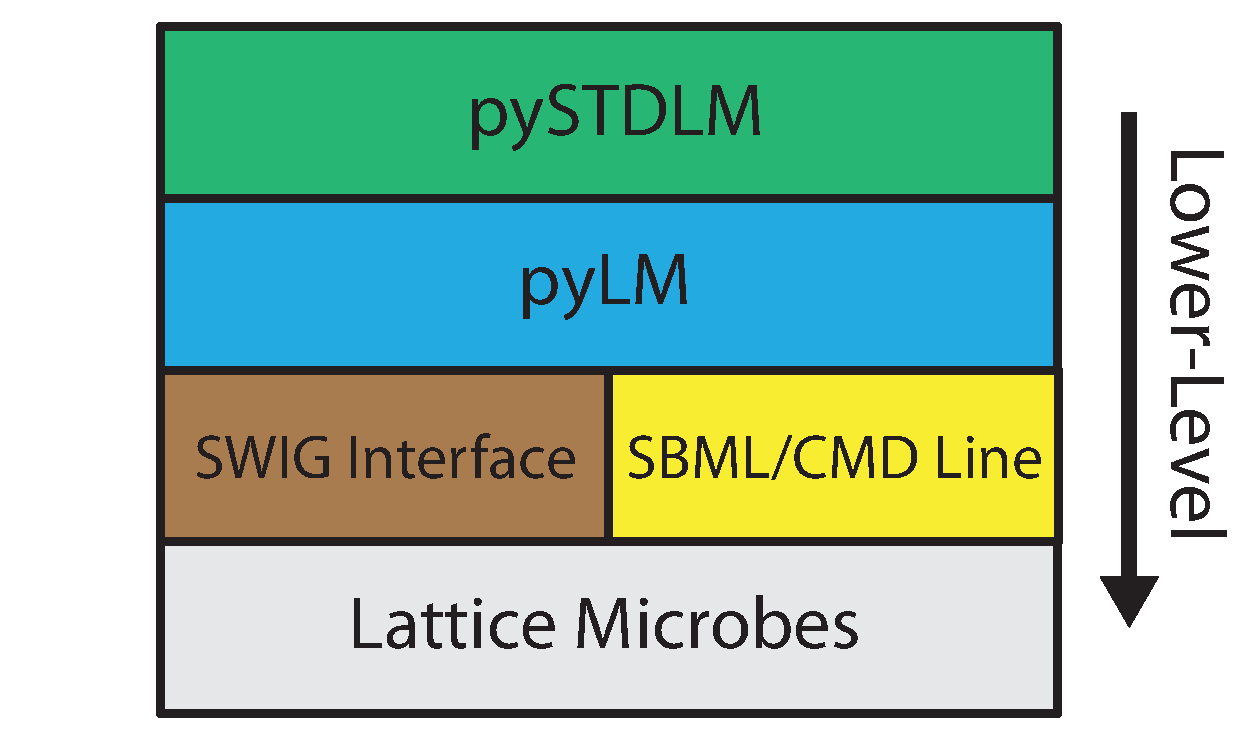
\includegraphics[width=0.7\textwidth]{Figures/Schematic.pdf}
  \caption{A schematic of the pyLM and the Lattice Microbes software.} \label{fig:pyschematic}
\end{figure}

The PSE is shown schematically in Figure \ref{fig:pyschematic}.  It sits on top of a SWIG interface that allows the C++ code to be accessible from the Python terminal.  Using pyLM allows the user to set up, run and post-process simulations all within a single script.  A general workflow is shown in Figure \ref{fig:workflow}.  For tutorials on using pyLM please see the ``pyLM Tutorial" and for in-depth description of all pyLM functionality please see the documentation ``pyLM Documentation".

\begin{figure}[h!]
  \centering
      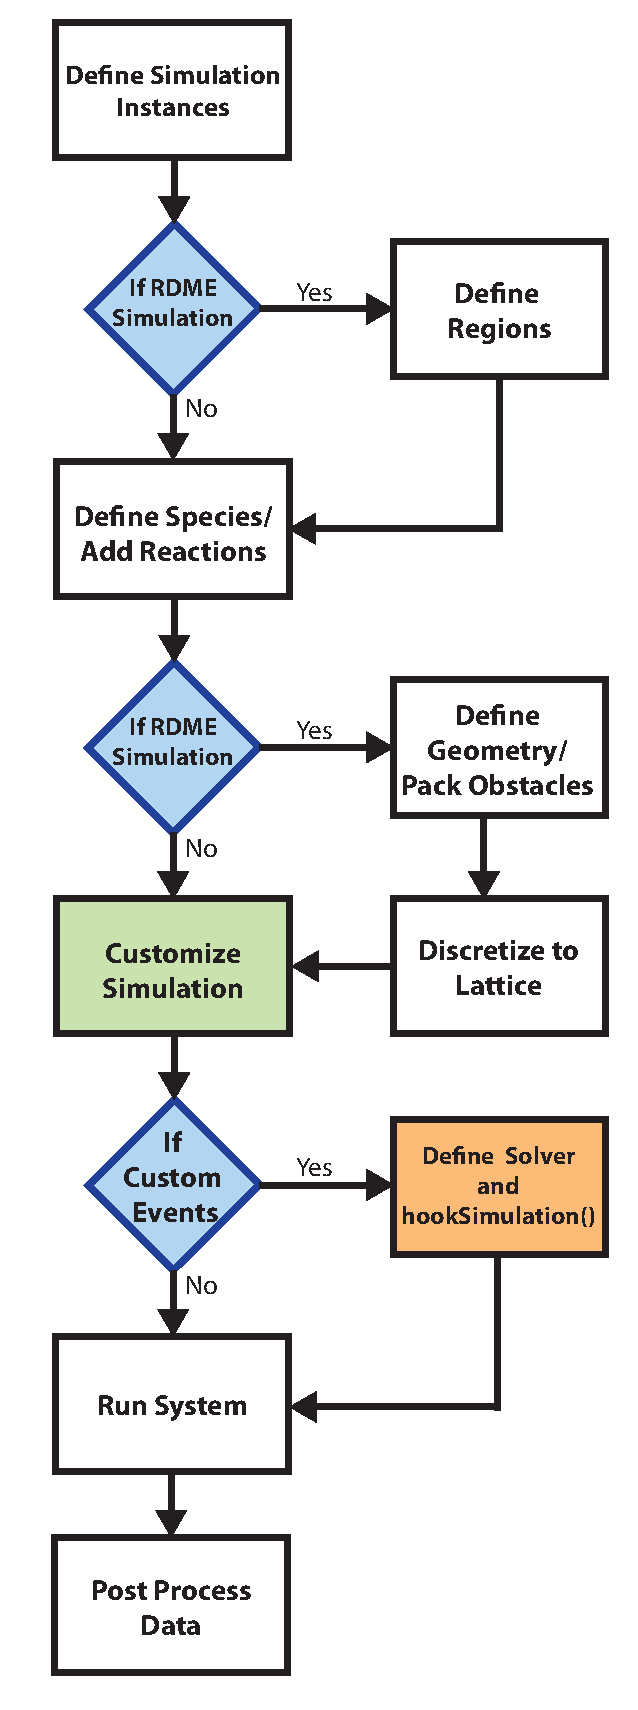
\includegraphics[width=0.5\textwidth]{Figures/Workflow.pdf}
  \caption{The workflow of the pyLM PSE.} \label{fig:workflow}
\end{figure}

%%%%%%%%%%
% Section: Stochastic Modeling %
%%%%%%%%%%
\section{Stochastic Modeling}

Lattice Microbes can be used to simulate chemical master equations (CME):
\begin{equation*}
\frac{dP(\mathbf{x},t)}{dt}=\sum_{r}^{R} [-a_r({{\mathbf{x}}}) P({{\mathbf{x}}},t) + a_r({{\mathbf{x}}}_\nu-\mathbf{S_r}) P({{\mathbf{x}}}-\mathbf{S_r},t)]
\end{equation*}

\noindent and reaction-diffusion master equations (RDME):
\begin{align*}
\frac{dP(\mathbf{x},t)}{dt}=\sum_{\nu}^{V}\sum_{r}^{R} &[-a_r({{\mathbf{x}}}_\nu) P({{\mathbf{x}}}_\nu,t) + a_r({{\mathbf{x}}}_\nu-\mathbf{S_r}) P({{\mathbf{x}}}_\nu-\mathbf{S_r},t)]\\
+\sum_{\nu}^{V}\sum_{\xi}^{\pm\hat{i},\hat{j},\hat{k}}\sum_{\alpha}^{N} &[-d^{\alpha} x_{\nu}^{\alpha} P({{\mathbf{x}}},t) + d^{\alpha} (x_{\nu+\xi}^{\alpha}+1_{\nu}^{\alpha}) P({{\mathbf{x}}}+1_{\nu+\xi}^{\alpha}-1_{\nu}^{\alpha},t)]
\end{align*}

\noindent using a variety of methods.

%%%%%%%%%%
% Section: Capabilities %
%%%%%%%%%%
\section{Capabilities}
pyLM and the included library of standard systems pySTDLM provide a problem solving environment for setting up, running and analyzing stochastic biological simulations \cite{Peterson2013}.  It contains functionality for specifying simulation setup including:

\begin{itemize}
\item Named species
\item Initial counts and distributions 
\item Reactions and rates
\item Spatial localization and definition
\item Diffusion properties
\item Obstacles
\item Handles to data in the popular Numpy array representation
\item Plotting species averages/variances and individual time traces
\item Plotting Kymographs of spatial species distributions
\item Reaction network generation
\item Dynamic reaction network representations
\end{itemize}

